\documentclass{article}
\usepackage[spanish]{babel}
\usepackage[numbers,sort&compress]{natbib}
\usepackage{graphicx}
\usepackage{url}
\usepackage{amsmath}
\usepackage{hyperref}
\usepackage{float}
\usepackage{color}
\definecolor{gray86}{gray}{.86}
\definecolor{gray75}{gray}{.75}
\definecolor{gray45}{gray}{.45}
\usepackage{listings}
\lstset{ 
language=C,                
basicstyle=\footnotesize,      
numbers=left,                  
numberstyle=\footnotesize,     
stepnumber=1,                   
numbersep=5pt,                  
backgroundcolor=\color{gray86},  
showspaces=false,              
showstringspaces=false,         
showtabs=false,                
frame=single,           
tabsize=2,          
captionpos=b,          
breaklines=true,        
breakatwhitespace=false,   
escapeinside={\%*}{*)}          
}
\usepackage{subfigure} 
\usepackage[top=15mm, bottom=15mm, left=15mm, right=15mm]{geometry}
\setlength{\parskip}{2mm}
\setlength{\parindent}{0pt}

\author{Abraham Azael Morales Juárez  1422745}
\title{Interacciones entre partículas}
\date{\today}

\begin{document}

\maketitle

\section{Introducción}
En está práctica se realizará un modelo simplificado para los fenómenos de atracción y resulsión, uno de estos fenómenos se le conoce fuerza electrostática\cite{REF1}. En donde aplica la ley de Coulomb, partículas con cargas iguales se repelen y con cargas opuestas se atraen. Además de que su fuerza es proporcional a la diferencia de la magnitud de las cargas e inversamente proporcional a la distancia euclidiana entre las partículas. Se crearán partículas, que tendrán estás características de atracción o repulsión\cite{REF2}.
\section{Objetivos}
Agregar a cada partícula masa y generar que esta masa afecte las fuerzas de atracción.\\
Estudiar la distribución de las velocidades de las partículas y verificar que este presente una relación entre los factores: velocidad, carga y masa.

\section{Resultados}
En la figura 1 se observan los resultados de las 50 partículas generadas donde el color representa la magnitud de la carga. 
\begin{figure}[H]
\centering
\includegraphics[width=9cm]{p9i.png}
\caption{Partículas generadas.}
\end{figure}
En el código se agregaron los parámetros con los cuales se trabajo, entre ellos la variable nueva que es la masa.
\begin{lstlisting}[frame=single]
n <- 50
p <- data.frame(x = rnorm(n), y=rnorm(n), c=rnorm(n), m=rnorm(n))
mmax <- max(p$m)
mmin <- min(p$m)
p$m <- ((p$m - mmin)*(p$m - mmin) / (mmax - mmin))+1 
xmax <- max(p$x)
xmin <- min(p$x)
p$x <- (p$x - xmin) / (xmax - xmin) # ahora son de 0 a 1
ymax <- max(p$y)
\end{lstlisting}
Además se agregan las líneas del código donde estas muestran el efecto que tienen sobre las fuerzas de atracción entre las partículas así cómo la velocidad de estas.

\begin{lstlisting}[frame=single]
fuerzas <- data.frame()
for (iter in 1:tmax) {
  aux <- c()
  f <- foreach(i = 1:n, .combine=c) %dopar% fuerza(i)
  delta <- 0.02 / max(abs(f)) # que nadie desplace una paso muy largo
  mf <- delta*f
  p$x <- foreach(i = 1:n, .combine=c) %dopar% max(min(p[i,]$x + delta * f[c(TRUE, FALSE)][i], 1), 0)
  p$y <- foreach(i = 1:n, .combine=c) %dopar% max(min(p[i,]$y + delta * f[c(FALSE, TRUE)][i], 1), 0)
  for(t in seq(1, (length(mf) -1), by = 2)){
    aux <- c(aux, (sum((mf[t])^2, (mf[t +1])^2))^(1/2))
  }
  fuerzas <- rbind(fuerzas, aux)
  tl <- paste(iter, "", sep="")
  while (nchar(tl) < digitos) {
    tl <- paste("0", tl, sep="")
  }
\end{lstlisting}
En la figura 2 y 3 se puede observar el comportamiento de estas partículas a lo largo del experimento, tomando como ejemplos distintas etapas para poder observar mejor el avance de estas.
\begin{figure}[H]
\centering
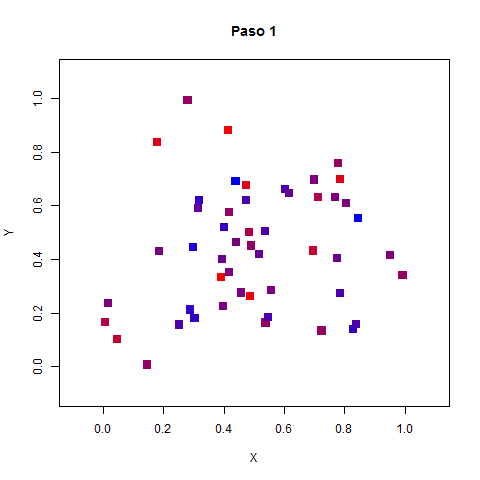
\includegraphics[width=7cm]{p9_t001.png}  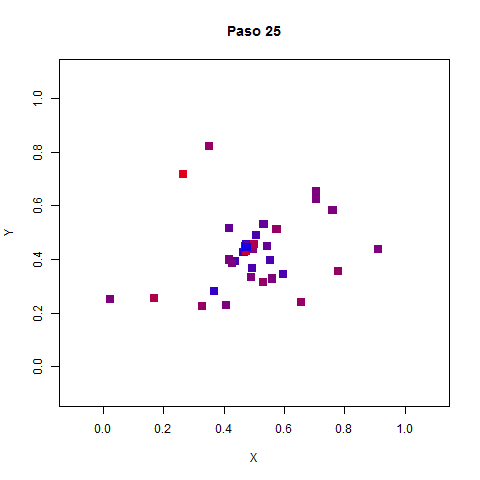
\includegraphics[width=7cm]{p9_t025.png} 
\caption{Simulación de atracción de las partículas en los pasos 1 y 25.}
\end{figure}
\begin{figure}[H]
\centering
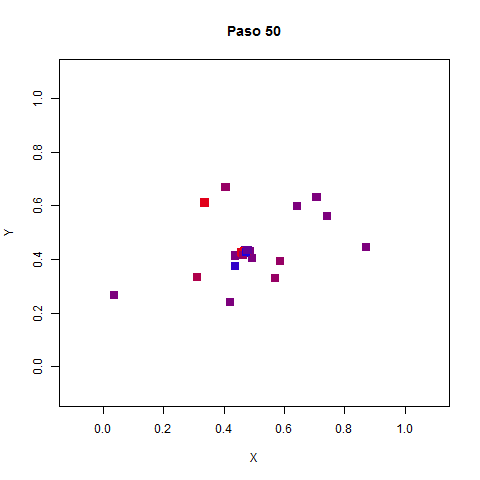
\includegraphics[width=7cm]{p9_t050.png} 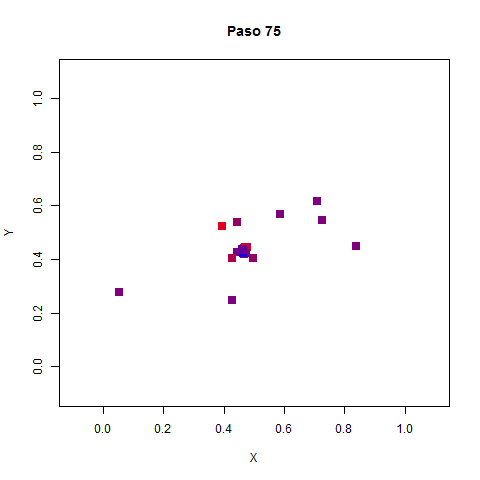
\includegraphics[width=7cm]{p9_t075.png}
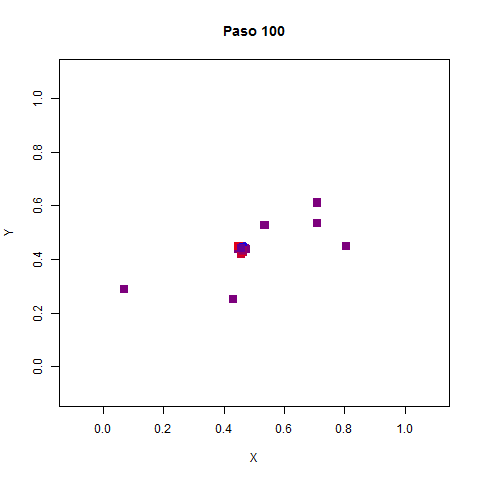
\includegraphics[width=7cm]{p9_t100.png}
\caption{Simulación de atracción de las partículas en los pasos 50, 75 y 100.}
\end{figure}
De la figura 4 - 7 se muestran las velocidades de distintas secciones del experimento, y estas observando que van obteniedo la misma velocidad conforme avanzan los pasos.
\begin{figure}[H]
\centering
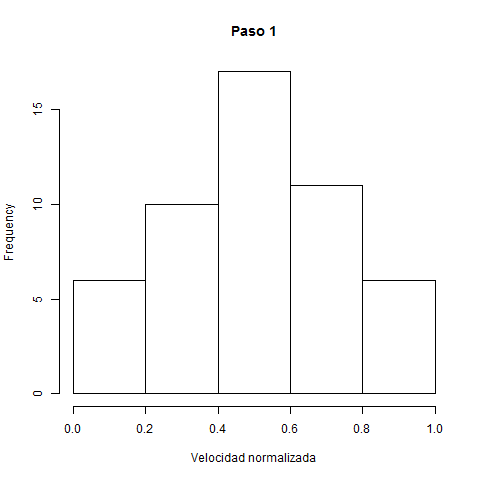
\includegraphics[width=7cm]{histx_001.png} 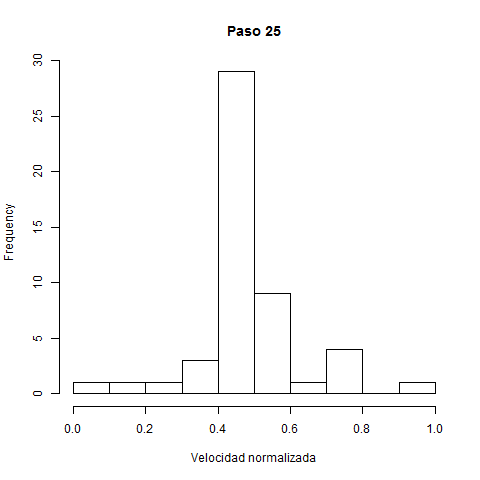
\includegraphics[width=7cm]{histx_025.png}
\caption{Velocidad de las partículas con respecto al eje X para el paso 1 y 25}
\end{figure}
\begin{figure}[H]
\centering
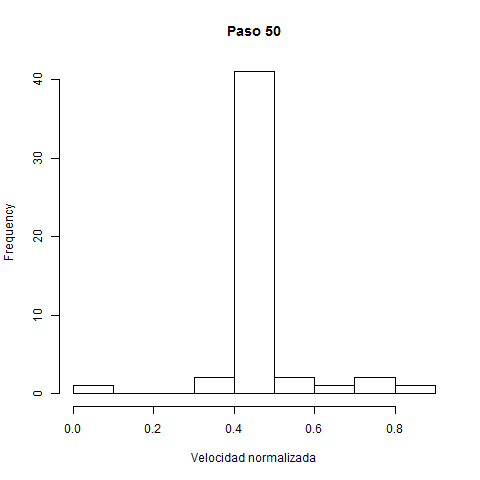
\includegraphics[width=7cm]{histx_050.png} 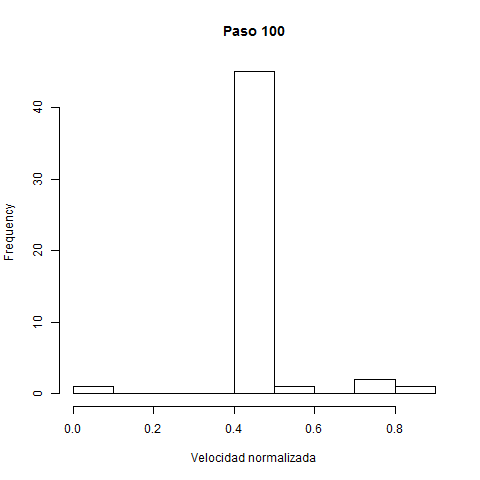
\includegraphics[width=7cm]{histx_100.png}
\caption{Velocidad de las partículas con respecto al eje X para el paso 50 y 100}
\end{figure}

\begin{figure}[H]
\centering
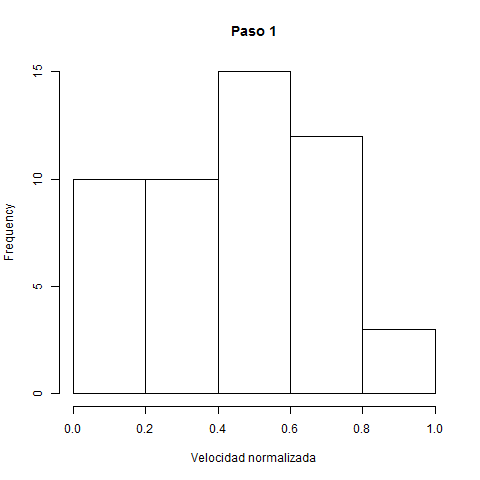
\includegraphics[width=7cm]{histy_001.png} 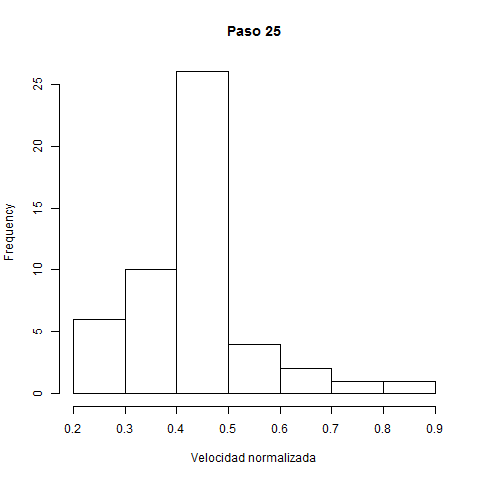
\includegraphics[width=7cm]{histy_025.png}
\caption{Velocidad de las partículas con respecto al eje Y para el paso 1 y 25}
\end{figure}
\begin{figure}[H]
\centering
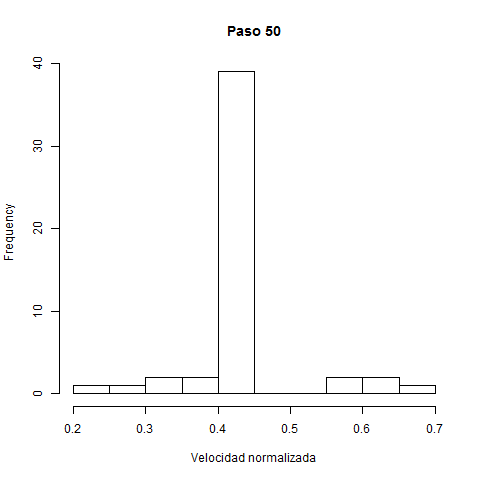
\includegraphics[width=7cm]{histy_050.png} 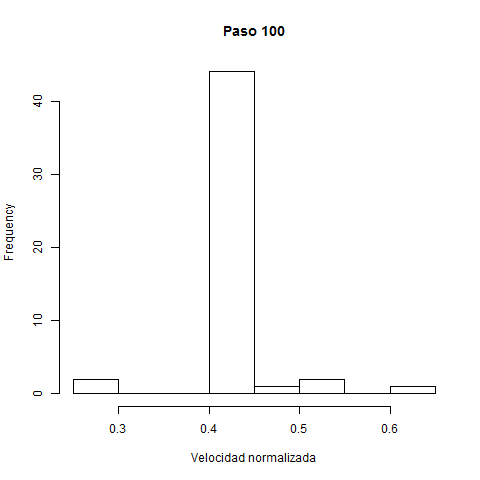
\includegraphics[width=7cm]{histy_100.png}
\caption{Velocidad de las partículas con respecto al eje Y para el paso 50 y 100}
\end{figure}

En la figura 8 y 9 se observa la relación existente entre las variables que se tienen. Se aplicó la función pairs para obtener las gráficas.
Se pudó determinar una relación existente entre la velocidad de X y Y por ese motivo se puede observar este tipo de comportamiento a lo largo de este experimento. Y también se observó que con las variables de carga y masa no presentan una relación, por eso la gráfica con el paso del tiempo no tuvo cambio alguno.

\begin{figure}[H]
\centering
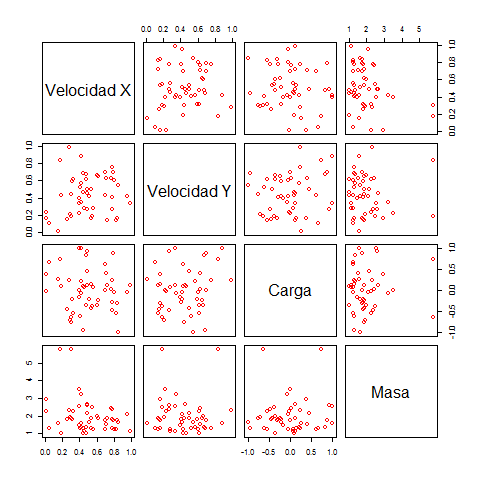
\includegraphics[width=7cm]{relacion_para_atraccion001.png} 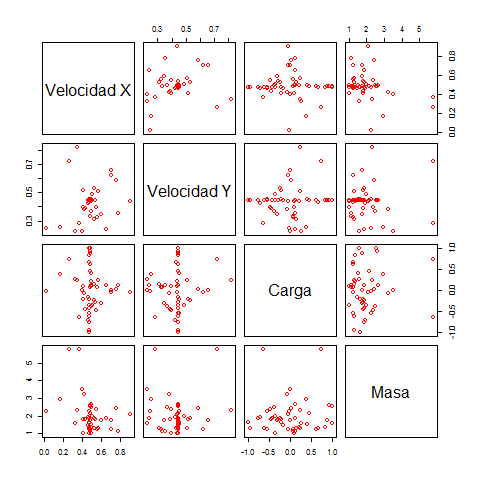
\includegraphics[width=7cm]{relacion_para_atraccion025.png}
\caption{Relación entre las diferentes variables, paso 1 y 25}
\end{figure}

\begin{figure}[H]
\centering
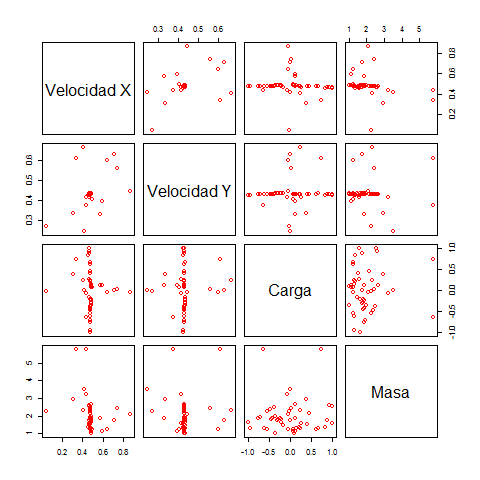
\includegraphics[width=7cm]{relacion_para_atraccion050.png} 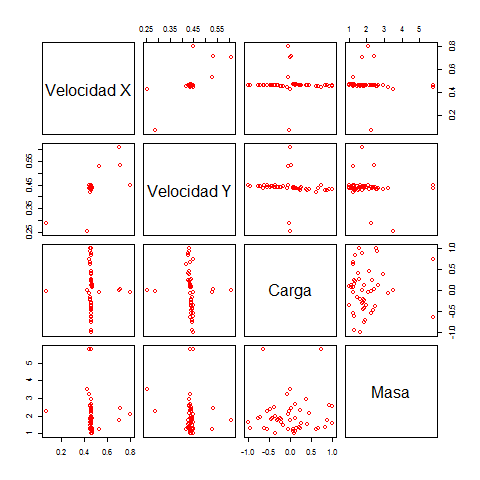
\includegraphics[width=7cm]{relacion_para_atraccion100.png}
\caption{Relación entre las diferentes variables, paso 50 y 100}
\end{figure}


\section{Conclusiones}
Sin importar la masa de las partículas estan llegan a juntarse y mantenerse estables.\\
Se pudo apreciar que no hubo una relación entre la masa y la carga de las partículas y que no afecto de manera negativa a las demás variables.

\bibliographystyle{plainnat}
\bibliography{ref9}




\end{document}